\documentclass[a4paper,UKenglish]{lipics-v2018}
\usepackage{microtype}%if unwanted, comment out or use option "draft"
\bibliographystyle{plainurl}% the recommnded bibstyle

\title{Formal Methods for Security - Final Report}

\author{Daniel Schaefer}{2549458}{}{}{}
\authorrunning{Daniel Schaefer}
\renewcommand{\copyrightline}{}

\begin{document}
\maketitle

\begin{abstract}
In this course we generally talked about various methods of model-checking security protocols. Later on here should be a text that summarizes the idea and findings of the seminar.\\
% TODO Extend

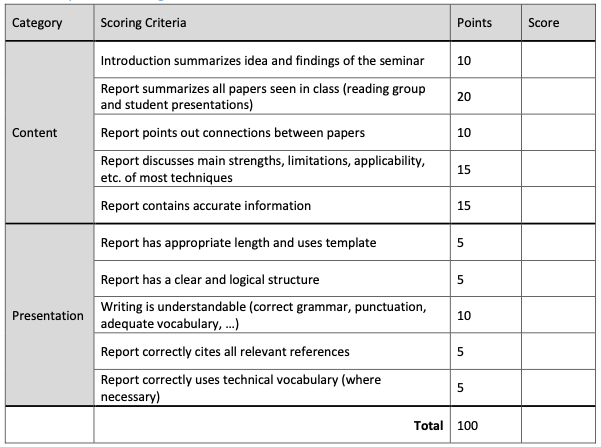
\includegraphics[scale = 0.72]{pictures/grading_scheme}\\
\end{abstract}


\section{Model Checking Security Protocols}
% TODO


\section{Language Based Information Flow Security}
% TODO



\section{Secure Information flow by self-composition}
% TODO



\section{Automated Analysis of Cryptographic Protocols using Murphi}
% TODO



\section{SAT based model-checking for security protocol analysis}
% TODO



\section{Automatic Verification of Security Protocols in the Symbolic Model: the Verifier ProVerif}
Example citation \cite{ProVerif}
% TODO



\bibliography{finalReport}


\end{document}
